%%%%%%%%%%%%%%%%%%%%%%%%%%%%%%%%%%%%%%%%%%%%%%%%%%%%%%%%%%%%%%%%%%%%%%%%%%%%%%%%
% Anonymous ICRA 2027 submission draft.
% Official Papercept ieeeconf.cls, US Letter, 10 pt, conference mode.
%%%%%%%%%%%%%%%%%%%%%%%%%%%%%%%%%%%%%%%%%%%%%%%%%%%%%%%%%%%%%%%%%%%%%%%%%%%%%%%%
\documentclass[letterpaper,10pt,conference]{ieeeconf}

\IEEEoverridecommandlockouts
\overrideIEEEmargins

\usepackage{graphicx}
\usepackage{amsmath,amssymb}
\usepackage{booktabs}
\usepackage{array}
\usepackage{cite}
\usepackage{url}
\usepackage{xcolor}
\usepackage{balance}

\graphicspath{{figures/}}
\newcommand{\methodgng}{GNG}
\newcommand{\methodguard}{Guarded GNG}
\newcommand{\methodhalton}{Halton/PRM}
\newcommand{\pp}{\,pp}
\renewcommand{\arraystretch}{1.08}

\title{\LARGE \bf
Configuration-Retaining Reachability Roadmaps for\\
Dual-Topology Manipulation under Environment Updates
}

% ICRA 2027 uses double-anonymous review. Author identities and affiliations
% must be restored only after acceptance.
\author{Anonymous Authors}

\begin{document}
\maketitle
\thispagestyle{empty}
\pagestyle{empty}

\begin{abstract}
We present a preview-only manipulation-planning architecture that intersects an environment graph containing semantic targets and obstacle primitives with a robot reachability graph whose nodes retain complete six-joint configurations. Candidate routes are filtered by cached swept-body capsules and then validated at interpolated states with MoveIt/FCL; rejected edges are disabled within the query and graph search repeats. We compare three 800-node constructions under shared connection and collision rules: a Growing Neural Gas (GNG)-quantized $k$-nearest-neighbor roadmap, a guarded hybrid with two anchors, 199 GNG prototypes, and 599 deterministic low-discrepancy samples, and a Halton/PRM baseline. A frozen controller-free evaluation spans 60 deterministic roadmap streams and 30 base trajectories crossed with point and segment obstacles, totaling 180 graph builds and 21,600 clear/dynamic queries. All integrity contracts passed. Dynamic exact-valid success was 73.8\% for GNG, 77.4\% for guarded GNG, and 80.5\% for Halton/PRM. Guarded GNG improved the prespecified risk difference over GNG by $3.7\pp$ (fixed-catalog 95\% CI $[1.6,5.8]$; Holm-adjusted permutation $p=.0032$), but remained $3.1\pp$ below Halton/PRM (CI $[-5.2,-0.9]$; $p=.0088$). Thus, deterministic guards mitigate a pure-GNG local-support failure but do not establish superiority over low-discrepancy sampling.
\end{abstract}

\section{Introduction}
A Cartesian target is not automatically executable. Multiple inverse-kinematic branches may reach nearby end-effector positions, yet only some connect collision-free to the measured arm state. Capability maps summarize workspace access~\cite{zacharias2007,porges2014}, whereas probabilistic roadmaps (PRMs) amortize configuration-space search~\cite{kavraki1996}. Manipulation under evolving RGB-D observations needs both: semantic target selection in workspace and persistent validated connectivity in configuration space.

We study a dual-topology architecture. The environment graph $G_E$ represents target-labeled nodes and obstacle-bearing nodes or edges. The robot graph $G_R$ represents collision-valid configurations, end-effector poses, and validated local transitions. A target becomes actionable only when an overlapping robot node belongs to the component connected to the current configuration. The implementation publishes a trajectory preview on a private topic and exposes neither a controller publisher nor a \texttt{FollowJointTrajectory} action client.

The initial motivation was to learn configuration-space topology with GNG~\cite{fritzke1995}. Implementation audit revealed that the current planner retains GNG prototypes but discards learned GNG adjacency before rebuilding every method with a shared validated $k$-nearest-neighbor rule. We therefore use the precise term \emph{GNG-quantized PRM}, not topology-preserving GNG. This paper contributes:
\begin{itemize}
    \item a typed dual-topology planner that retains full joint configurations and multiple kinematic branches behind end-effector positions;
    \item cached full-body capsule invalidation followed by lazy interpolated MoveIt/FCL validation and within-query edge rejection;
    \item an auditable guarded-GNG construction under a fixed 800-node budget; and
    \item a provenance-bound 60-stream, 60-scene benchmark that quantifies where guarding helps and where Halton/PRM remains stronger.
\end{itemize}

\section{Related Work}
PRMs separate roadmap construction from repeated queries~\cite{kavraki1996}. Low-discrepancy sequences provide deterministic space-filling alternatives to pseudorandom samples~\cite{branicky2001}. Sparse roadmap spanners and experience graphs reduce or reuse graph structure~\cite{dobson2014,phillips2012,coleman2015}. Our graph is a persistent configuration-space roadmap rather than a binary reachability volume: nearby end-effector positions may retain distinct joint branches and transitions, but the method provides no asymptotic optimality or completeness guarantee.

Lazy PRM postpones expensive checks to query time~\cite{bohlin2000}. Dynamic Roadmaps and changing-environment PRMs cache or update workspace-to-roadmap influence~\cite{kallmann2004,jaillet2004}. Our capsule cache is a conservative broad phase before exact FCL validation. Learned samplers can focus computation~\cite{ichter2018,qureshi2019,chamzas2021}, while globally supportive samples can hedge against concentration. Guarded GNG is one deterministic hybrid, not a probabilistic-completeness claim.

\section{Problem Formulation}
Let $Q$ be the six-dimensional joint-limit box and $Q_{\mathrm{free}}$ the configurations accepted by kinematic and collision predicates. Robot node $v_i$ stores joint vector $q_i$, its range-normalized form, and end-effector pose $x_i=\mathrm{FK}(q_i)$. Normalized joint distance is
\begin{equation}
d_Q(q_i,q_j)=\sqrt{\sum_k\left(\frac{q_{i,k}-q_{j,k}}
{q_k^{\max}-q_k^{\min}}\right)^2}.
\label{eq:dq}
\end{equation}
The world-frame environment graph $G_E=(V_E,E_E)$ partitions semantic targets $T$ from point or segment obstacles $O$. Given target $t$ and start $q_s$, candidate intersections are
\begin{equation}
\mathcal{I}(t)=\{v_i\in V_R:\lVert p_i-p_t\rVert_2\le r_I,
\ v_i\ \mathrm{free},\ v_i\leftrightarrow v_s\}.
\label{eq:intersection}
\end{equation}
Dijkstra search minimizes accumulated joint-space roadmap cost to a node in $\mathcal{I}(t)$. A preview is exact-valid only when every interpolated state passes detailed robot and environment collision checks. Time parameterization, dynamics, controller tracking, and moving-obstacle prediction are outside the current interface.

\section{Dual-Topology Planner}
\begin{figure*}[t]
    \centering
    
\includegraphics[width=0.96\textwidth]{system_architecture.png}
    \caption{Dual-topology pipeline. Environment targets intersect configuration-retaining robot nodes; cached capsule invalidation precedes lazy MoveIt/FCL route validation. Output remains preview-only.}
    \label{fig:architecture}
\end{figure*}

\subsection{Environment and Robot Graphs}
In the full system, a wrist-mounted RealSense D405 supplies a world-frame point cloud to DD-GNG. Stable environment nodes retain position, semantic class, confidence, and edges. Target-labeled nodes become goal hypotheses; non-target nodes and segments become collision primitives, with a small exclusion around the selected target. Perception and reachability are separate ROS~2 processes, so roadmap experiments run without opening the camera or launching hardware interfaces. The experiments reported here inject synthetic oracle-validated environments and do not evaluate perception.

\subsection{Node-Budget-Matched Roadmaps}
All methods begin with two fixed anchors and end at exactly 800 nodes. Pure GNG trains on 4,000 valid normalized configurations and retains 798 prototypes. Guarded GNG retains 199 prototypes and adds 599 deterministic raw valid samples selected across the same candidate stream. Halton/PRM adds 798 digit-permuted Halton samples directly. Every method then uses the same validated $k$-nearest-neighbor connection stage. The comparison matches final node count, joint limits, local rules, and collision predicates, but not candidate information or computation: both GNG variants inspect 4,000 accepted training configurations, whereas Halton directly fills its graph.

\subsection{Broad-Phase Invalidation and Exact Replanning}
Roadmap nodes and interpolated edges cache capsules spanning the arm, end effector, fingers, and camera payload. Point-to-segment and segment-to-segment distances invalidate candidates without rebuilding the roadmap:
\begin{equation}
\operatorname{blocked}(c,o)\iff d(\operatorname{axis}(c),o)<r_c+\delta,
\label{eq:block}
\end{equation}
where $r_c$ is capsule radius and $\delta$ is clearance. A surviving route is reconstructed in a MoveIt PlanningScene~\cite{coleman2014} and checked with FCL~\cite{pan2012}. If exact validation rejects an edge, that edge is disabled for the environment and Dijkstra search repeats, up to 20 times. Query responses echo scene, stream, method, graph revision, target, start state, validity flags, and diagnostic counters; stale or mismatched responses are rejected.

\section{Experimental Protocol}
\subsection{Implementation and Safety Boundary}
The ROS~2 Humble C++ implementation runs on an NVIDIA Jetson AGX Orin. MoveIt RobotModel/RobotState provide kinematics and self-collision state; PlanningScene and FCL validate detailed meshes. Isolated localhost-only ROS domains launch neither MoveGroup, \texttt{ros2\_control}, a camera process, nor controller endpoints. Preflight requires a clean domain and exactly one expected graph publisher, plan publisher, and query subscriber.

\begin{table}[t]
\caption{Frozen roadmap and query parameters.}
\label{tab:parameters}
\centering
\scriptsize
\setlength{\tabcolsep}{3pt}
\begin{tabular}{@{}lcl@{}}
\toprule
Parameter & Value & Role \\
\midrule
Nodes / GNG signals & 800 / 4000 & node / training budget \\
Guard composition & 0.75 & 2 anchor + 199 GNG + 599 guard \\
$k$ / max. $d_Q$ & 10 / 0.75 & shared connection rule \\
Max. Cartesian edge & 0.14 m & local displacement \\
Target radius $r_I$ & 0.05 m & graph intersection \\
Clearance & 0.035 m & capsule margin \\
Point / segment radius & 0.012 / 0.006 m & environment geometry \\
Body / exact step & 0.08 / 0.05 & broad / exact interpolation \\
\bottomrule
\end{tabular}
\end{table}

\subsection{Evidence Separation and Frozen Design}
Offsets 0--49 exposed eight pure-GNG failures and selected the 75\% guard fraction. Offsets 50--99 then evaluated one anchored task, and a six-stream, six-scene smoke verified atomic queries and analysis plumbing. Because these stages informed the final instrumentation, neither is pooled with confirmatory inference.

The frozen \texttt{om6dof\_icra\_scene\_catalog\_v4} contains 30 deterministic base start--target trajectories, each crossed with point and segment obstacles. Ten bases belong to each low-, medium-, and high-difficulty stratum. An independent oracle accepts a scene only when the clear direct interpolation is valid, the dynamic obstacle blocks it under capsule and exact checks, endpoints and a detour state remain valid, and the two-leg detour is collision-free.

Stream labels 100--159 are fixed deterministic digit-permuted Halton keys, not ordinary random seeds. The six method orders occur ten times each. Scene order is rotated identically across methods, and clear/dynamic phase order is parity-counterbalanced. The design yields $60$ streams $\times 3$ methods $\times 60$ scenes $\times 2$ phases $=21{,}600$ queries.

\subsection{Confirmatory Statistics}
The primary endpoint is dynamic exact-valid success. For each guarded-versus-baseline pair,
\begin{equation}
d_s=\frac{1}{60}\sum_j(Y_{g,s,j}-Y_{b,s,j}),\qquad
\Delta=\frac{1}{60}\sum_s d_s.
\label{eq:estimand}
\end{equation}
Only guarded-minus-GNG and guarded-minus-Halton are confirmatory; Holm correction covers exactly these hypotheses. Uncertainty uses 50,000 paired whole-stream bootstrap resamples with shared indices. A two-sided studentized sign-flip test flips the complete 60-scene method-difference vector per stream for 100,000 Monte Carlo draws. The primary interval is conditional on the fixed catalog. Success-conditional latency and cost use joint-success cells; path change requires common clear-and-dynamic success.

\section{Results}
All 180 graph builds and 21,600 queries passed correlation, provenance, target/start echo, validity-agreement, and safety contracts; no timeout or infrastructure-error row occurred.

\begin{figure*}[t]
    \centering
    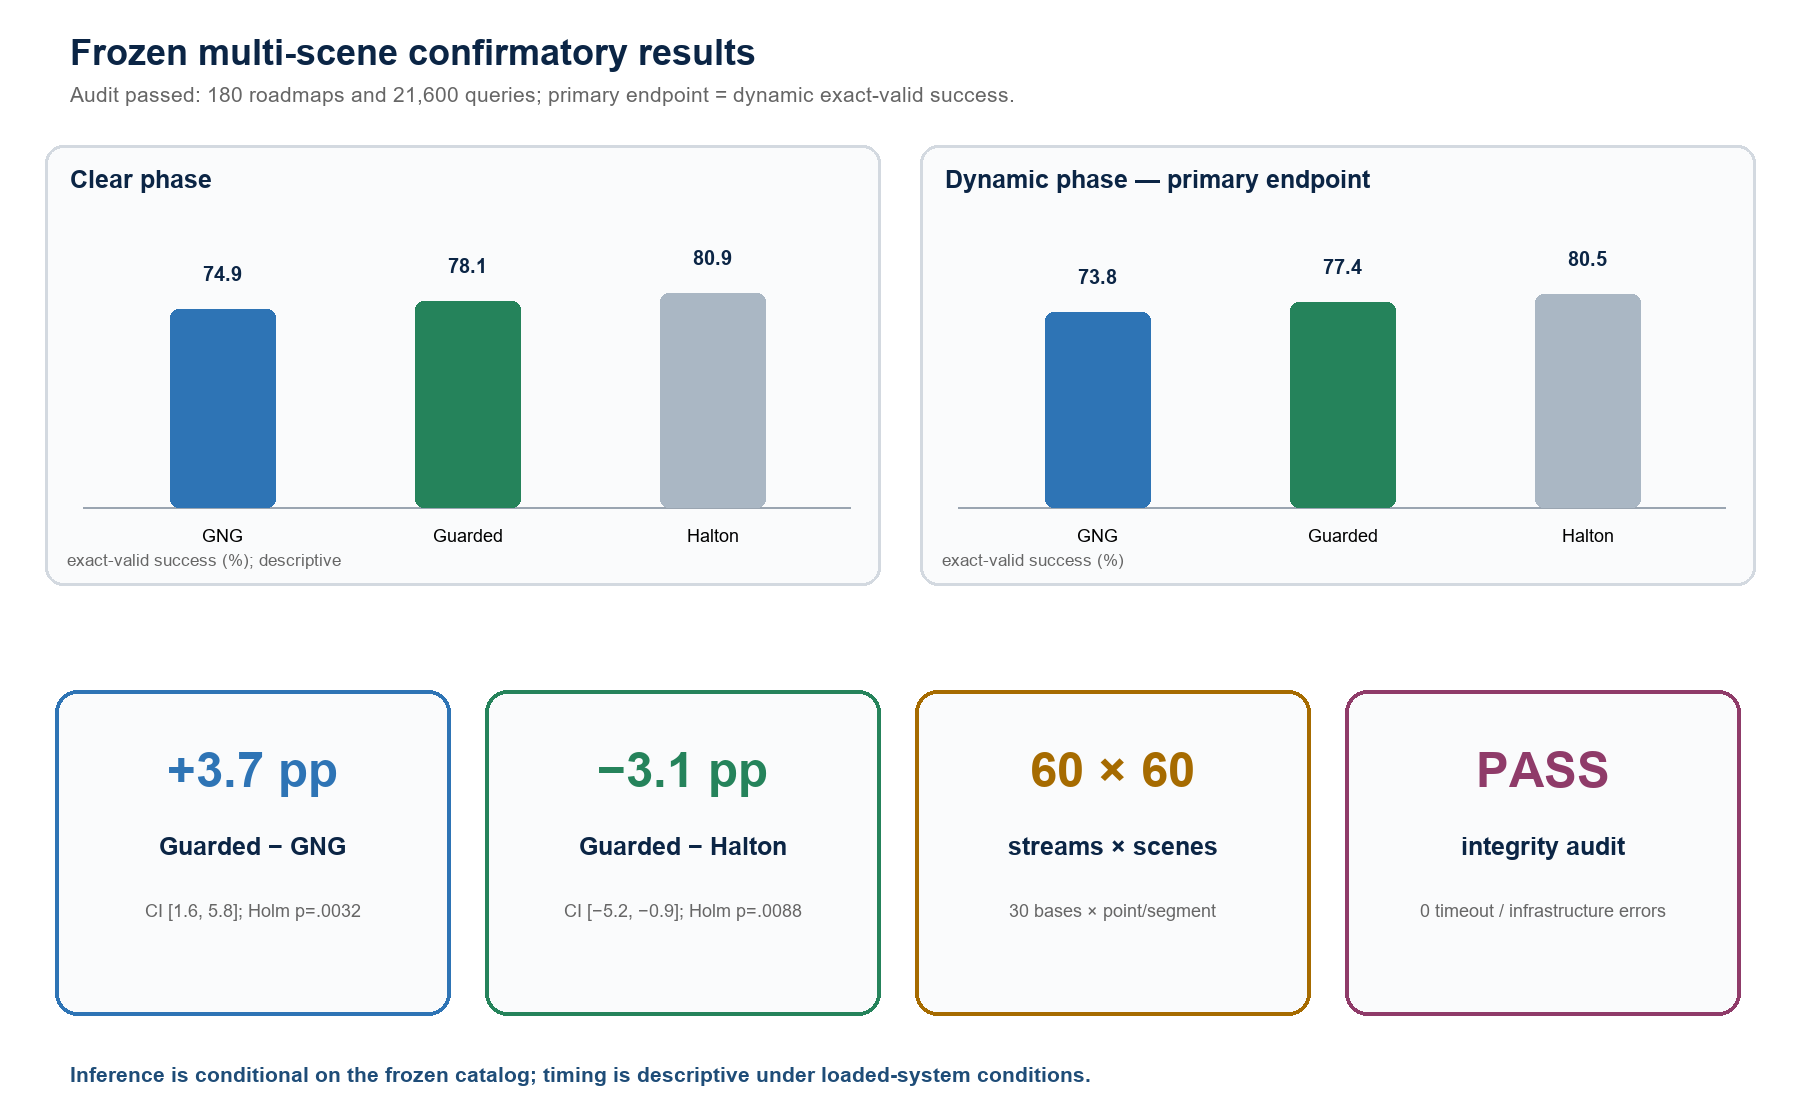
\includegraphics[width=0.96\textwidth]{confirmatory_results.png}
    \caption{Frozen multi-scene results. Guarded GNG improves dynamic exact-valid success over pure GNG, while Halton/PRM remains higher than guarded GNG. Inference is conditional on the fixed catalog.}
    \label{fig:results}
\end{figure*}

\begin{table*}[t]
\caption{Per-method results over 60 streams $\times$ 60 fixed scenes. Success intervals resample whole roadmap streams. Other values are descriptive; time and path-cost summaries use exact-valid paths only.}
\label{tab:methods}
\centering
\footnotesize
\resizebox{\textwidth}{!}{%
\begin{tabular}{@{}lccccccc@{}}
\toprule
Method & Clear success & Dynamic success & Retention & Build ms & Dynamic plan ms & Dynamic cost & Path change \\
\midrule
GNG & 74.9 [73.8,76.1]\% & 73.8 [72.6,75.0]\% & 98.4\% & 1721.5 [1708.1,1743.5] & 11.739 [8.504,18.820] & 12.227 [9.742,14.568] & 37.4\% \\
Guarded GNG & 78.1 [76.3,79.9]\% & 77.4 [75.7,79.2]\% & 99.1\% & 1594.1 [1576.6,1618.3] & 12.572 [9.220,19.791] & 14.835 [11.692,18.103] & 32.7\% \\
Halton/PRM & 80.9 [79.3,82.6]\% & 80.5 [78.9,82.1]\% & 99.5\% & 1393.8 [1377.7,1411.2] & 12.930 [9.318,19.153] & 15.665 [12.042,19.340] & 27.1\% \\
\bottomrule
\end{tabular}
}
\end{table*}

\subsection{Primary Endpoint}
Guarded GNG exceeded pure GNG by $3.7\pp$, and the paired whole-stream interval excluded zero. The stream-level sign-flip test remained significant after the prespecified Holm correction. Against Halton/PRM, guarded GNG was $3.1\pp$ lower, with an interval also excluding zero. Both null hypotheses were rejected in opposite directions: guarding mitigates pure GNG's local-support failure but does not outperform Halton/PRM.

\begin{table}[t]
\caption{Prespecified dynamic-success contrasts.}
\label{tab:primary}
\centering
\footnotesize
\begin{tabular}{@{}lccc@{}}
\toprule
Contrast & Risk diff. & Fixed-catalog 95\% CI & raw / Holm $p$ \\
\midrule
Guarded$-$GNG & $+3.7\pp$ & $[+1.6,+5.8]\pp$ & .0016 / .0032 \\
Guarded$-$Halton & $-3.1\pp$ & $[-5.2,-0.9]\pp$ & .0088 / .0088 \\
\bottomrule
\end{tabular}
\end{table}

\subsection{Secondary Outcomes}
Conditional clear-to-dynamic retention was high for all methods. Pure GNG returned the lowest median successful-path cost despite lower success coverage. Median build time was lowest for Halton/PRM and highest for pure GNG. Timing is descriptive because the AGX shared resources with background workloads and success-conditioned supports differ.

Point and segment obstacles produced similar guarded-minus-GNG effects ($+3.4$ and $+3.9\pp$). Descriptively, the effect concentrated in the high-difficulty stratum ($+9.7\pp$), while low and medium strata showed $+0.7$ and $+0.6\pp$. Guarded GNG remained below Halton/PRM in every reported difficulty stratum ($-2.8$ to $-3.2\pp$). These subgroup estimates were not multiplicity-tested.

\balance
\section{Reproducibility and Safety}
Frozen protocol v4 bound the catalog-generation contract, source snapshot, analyzer, and execution checklist before v4 outcomes. SHA-256 links the source manifest, catalog, protocol, runner, node, model inputs, raw rows, and logs. Runtime checks compare expanded URDF, SRDF, parameters, launch, messages, source, and node binary. Resume is fail-closed, and the deployed package completed 123 tests without failure. The benchmark is preview-only and cannot publish to a controller topic or trajectory action.

\section{Discussion and Limitations}
The confirmatory result separates global connectivity from target-conditioned support. Deterministic guards recover $3.7\pp$ relative to pure GNG, consistent with alternatives near target regions that adaptive quantization underrepresents. Yet Halton/PRM remains $3.1\pp$ higher, so the tested hybrid does not outperform direct low-discrepancy sampling at the same final node count. Pure GNG's lower successful-path cost suggests compact routes within the tasks it connects. A stronger successor should preserve or repair learned topology while protecting local target support, rather than globally increasing the guard fraction.

Primary intervals condition on the frozen catalog. A secondary stream-by-base-trajectory bootstrap widened guarded-minus-GNG to $[-2.7,+10.3]\pp$ and guarded-minus-Halton to $[-6.8,+0.6]\pp$; both include zero. Broader scene-population performance is therefore not established. Other limitations are synthetic obstacle geometry, position-dominant targets, unmatched candidate-information and compute budgets, absent RRTConnect/PRM*/SPARS comparisons, uncontrolled timing load, and no perception-in-the-loop or physical trajectory execution.

\section{Conclusion}
We presented a configuration-retaining, dual-topology reachability planner with fast capsule invalidation and lazy exact MoveIt/FCL validation. In a frozen 60-stream, 60-scene study, deterministic guards improved dynamic exact-valid success over pure GNG by $3.7\pp$, but remained $3.1\pp$ below Halton/PRM. The contribution is therefore not method superiority: guarding mitigates a local-support weakness of GNG quantization, while direct low-discrepancy sampling retains higher success under the tested node budget. Future work will study topology-aware local repair, controlled timing, perception-in-the-loop evaluation, and safety-approved physical execution.

\section*{AI Use Disclosure}
OpenAI Codex/ChatGPT assisted with manuscript drafting, LaTeX conversion, and figure preparation. The authors verified the implementation, numerical results, statistical interpretation, citations, and final claims.

\bibliographystyle{IEEEtran}
\bibliography{references}

\end{document}
